\chapter{Background \& Related Work}

This chapter introduces the core concepts built upon in this thesis and surveys
recent literature tackling the evaluation of generative graph neural networks
and the relevance of this problem in structural biology. Section
\ref{sec:background} defines core mathematical and biological concepts that will
be built upon in the thesis. Section \ref{sec:related} will discuss recent
advances in the design of measures used to evaluate generative graph neural
networks and in structural biology.

\section{Background}\label{sec:background}

The set of methods investigated in this thesis lies at the interface of
structural biology and machine learning. We start by defining some relevant
biological properties of proteins, followed by a survey various graph theoretical
abstractions derived from the protein structure. We then move on to define
generative models and the various classes of measures used to evaluate them.

\subsection{Proteins}\label{background:proteins}

Proteins are large biomolecules that are formed from a sequence of amino acids,
performing their functions as determined by their three-dimensional structure, and amino
acid sequence. Proteins support a vast array of functions in living organisms,
such as catalysing metabolic reactions, DNA replication, providing structural
support to cells, transporting molecules and sensing stimuli.

Each protein is made up of one or more chains of amino acids, each of which
contain a backbone and different side chains. The atoms in the backbone include
a \textalpha{}-carbon, another carbon and a nitrogen atom. An overview of the
peptide backbone is shown in Figure \ref{fig:backbone}. Interestingly, a plane
is forned by two alpha carbons, the carboxyl group, and the hydrogen atom attached
to the nitrogen atom (see Figure \ref{fig:backbone}), making the peptide bond
between the nitrogen and carbon atom resistant to twisting. That means that the
rotations enabling the 3D folding of a protein is governed by the angle of the bonds linking
the nitrogen atom to the \textalpha{}-carbon and the other carbon atom to the
\textalpha{}-carbon, named \textphi{} and \textpsi{}. These angles' values are
frequently used to validate proteins, characterise the secondary structure of proteins
(i.e. structural features observed in certain segments of proteins), etc.


\begin{figure}[h]
  \centering
  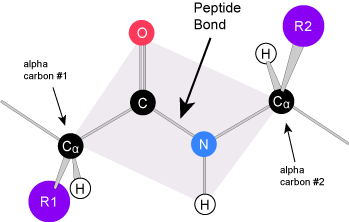
\includegraphics[width=.8\textwidth]{./figures/peptide_bond.png}
  \caption{Schematic of the backbone of a protein. Two \textalpha{}-carbons are
    shown as well as a \textbeta{}-carbon in the middle. R1 and R2 represent the
    side chains of the amino acid. }
  \label{fig:backbone}
\end{figure}


To visualize such angles, a Ramachandran plot can be constructed for any
protein. Such a plot can reveal secondary structural features such as
\textbeta{}-sheets, \textalpha{}-helices, etc. An example of such a plot together
with a 3D model of a protein can be found in Figure \ref{fig:ramachandran}.

\begin{figure}[h]
  \centering
  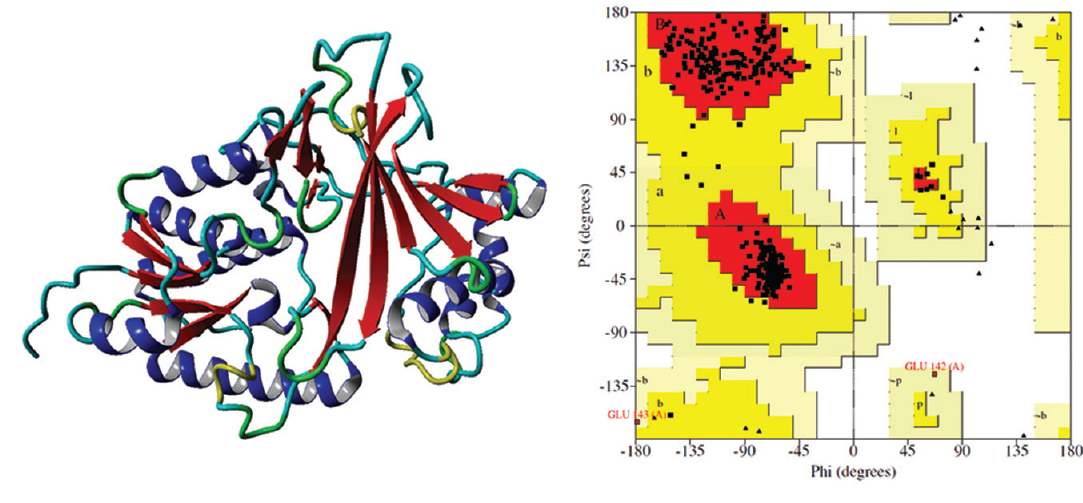
\includegraphics[width=.7\textwidth]{./figures/ramachandran_plot.jpg}
  \caption{3D structure of uridine diphosphogalactofuranose-galactopyranose
mutase with a corresponding Ramachandran plot. The \textalpha{}-helices can be
found on the middle left part of the Ramachandran plot, the \textbeta{} sheets on
the upper right quadrant, and the left handed \textalpha{}-helices can be found in
the middle upper right part of the plot. This figure is adapted from
\cite{nayak2018identification}.}
  \label{fig:ramachandran}
\end{figure}

\subsection{Graphs}

Proteins are often abstracted using graphs. A graph $G$ is a pair of vertices
$V$ and edges $E$ such that $G=(V, E)$, $|V|=n$ and $|E|=m$. Two vertices $i$
and $j$ are adjacent if there is an edge between them, i.e. $e_{ij}\in E$. The
relationship between between edges can be represented as an $n\times n$
adjacency matrix $A$, where:
\begin{equation}
  \label{eq:adjacency}
  A_{ij}=\begin{cases}
    1, \quad\text{if } e_{ij}\in E\\
    0, \quad\text{otherwise.}
  \end{cases}
\end{equation}
The neighborhood of a node $v$ is the set of nodes with an edge directly to $v$,
i.e. $N(v) = \{ u\in V|e_{uv} \in E \}$. A graph is undirected if the edges do
not contain directional information, i.e. $A_{ij}=A_{ji}$. A directed graph
would result in directionality being encoded in edges, where $A_{ij}$ would not
contain any information about $A_{ji}$. Nodes and edges in each graph can
contain one or more labels. In this thesis, we will mostly deal with labeled
undirected graphs, where each node will be labeled according to the amino acid
type each node belongs to.

There are multiple ways of constructing graphs from proteins. First, one can
extract a \emph{contact map} of a protein by computing the (euclidean) distance
between any two points belonging to each amino acid. The \textalpha-carbon is
often used for this purpose. This is a fully connected graph with continuously
labeled edges representing the distance between each node. From there, it is
possible to either extract a $k$-nearest neighbour graph, where
$k\in\mathbb{N}>0$ defines the amount of nodes directly connected to any given
nodes; or an $\varepsilon$-graph, where each node within a given distance
$\varepsilon\in\mathbb{R^+}\setminus \{0\}$ of another node is connected. Both
are graphs where each node is labeled with the residue name to which the
\textalpha{}-carbon belongs and the edges are unlabeled.

\subsection{Topological Data Analysis}

Although graphs are powerful abstractions of proteins, proteins can also be
represented as \emph{point clouds}. One powerful field of study of topological
properties of point clouds is \emph{topological data analysis}.

Topology has witnessed relentless theoretical progress since Henri Poincaré
first addressed topological ideas as a distinct branch of mathematics in his
1895 publication of \textit{Analysis Situs}~\citep{poincare1895analysis}. Only
recently, -- with the advent of modern computing -- has the field of
computational topology and topological data analysis (TDA) gained momentum to
investigate (high-dimensional) data in physics, biology, and
beyond~\citep{dey1999computational, ghrist2008barcodes, amezquita2020shape}. For
material providing an extensive and formal introduction to topology and
persistent homology, please refer to~\citep{freedman2009algebraic,
edelsbrunner2010computational}, and \citep{ghrist2008barcodes}.



\subsection{Generative models}

\subsection{Kernel methods}

\section{Related Work}\label{sec:related}

\subsection{Structural Biology}

\subsection{Metrics for Generative Graph Models}

\section{Summary}
